\documentclass[aspectratio=169]{beamer}

% --- THEME & COLORS ---
% Metropolis is a modern, minimalist theme suitable for tech/research
\usetheme{metropolis}
\metroset{block=fill} % Fills blocks with color for better visibility
\metroset{progressbar=frametitle} % Adds a subtle progress bar to slides

% Custom Colors (Professional Dark Slate & Teal aesthetics)
\definecolor{TechDark}{RGB}{35, 37, 43}
\definecolor{TechAccent}{RGB}{0, 150, 136} % Teal for emphasis
\setbeamercolor{frametitle}{bg=TechDark, fg=white}
\setbeamercolor{alerted text}{fg=TechAccent}
\setbeamercolor{progress bar}{fg=TechAccent, bg=TechDark!50}

% --- PACKAGES ---
\usepackage{graphicx}
\graphicspath{{images/}}
\usepackage{booktabs}
\usepackage{tikz}
\usetikzlibrary{shapes.geometric, arrows, positioning}
\usepackage{caption}

% --- META DATA ---
\title{Introduction to Computing at Scale}
\subtitle{The Design, Operation, and Societal Impacts of Data Centers}
\author{Max Hawkins}
\date{}
\institute{Georgia Institute of Technology} % Inferred from context or placeholder

\begin{document}

% --- TITLE SLIDE ---
\maketitle

% --- SECTION 1 ---
\section{Information \& Computing}

\begin{frame}{What is Information?}
    \centering
    \begin{quote}
        \Large ``Knowledge obtained from investigation, study, or instruction''
    \end{quote}
    \vspace{0.5em}
    \footnotesize{\textit{— Merriam-Webster}}

    \vspace{2em}
    \begin{columns}[T, onlytextwidth]
        \column{0.33\textwidth}
            \centering
            \textbf{Digital}\\
            Binary data in memory
        \column{0.33\textwidth}
            \centering
            \textbf{Algorithmic}\\
            Output of an algorithm
        \column{0.33\textwidth}
            \centering
            \textbf{Physical}\\
            Heat from a stove
    \end{columns}
\end{frame}

\begin{frame}{Information Processing is Valuable}
    % \textbf{Information Processing is Critical}

    \vspace{1.5em}
    \centering
    % Automated Diagram using TikZ
    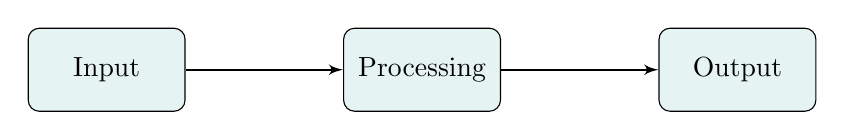
\begin{tikzpicture}[node distance=2cm, auto]
        \tikzstyle{block} = [rectangle, draw, fill=TechAccent!10,
            text width=5em, text centered, rounded corners, minimum height=3em]
        \tikzstyle{line} = [draw, -latex', thick]

        \node [block] (input) {Input};
        \node [block, right=of input] (process) {Processing};
        \node [block, right=of process] (output) {Output};

        \path [line] (input) -- (process);
        \path [line] (process) -- (output);
    \end{tikzpicture}

    \vspace{1.5em}
    \begin{itemize}
        \item \textbf{Biology:} Hunger $\to$ Look for food $\to$ Eat $\to$ Not hungry.
        \item \textbf{Umwelt:} How different species experience the world.
        \item \textit{Recommended Reading:} \emph{An Immense World} by Ed Yong.
    \end{itemize}
\end{frame}

\begin{frame}{Standardizing and Math}
    Humans have intuition (more vs. less or nothing), but precision and collaboration are needed.

    \begin{alertblock}{The Solution: MATH}
        Math serves as a common framework.
        \begin{itemize}
            \item \textbf{Standards} $\to$ Easier communication.
            \item Number systems, operations, written forms.
        \end{itemize}
    \end{alertblock}

    \vspace{1em}
    \textbf{Computation} = Information Processing + Math?
\end{frame}

\begin{frame}{Why We Need Computers}
    The human brain is \textbf{bad at math}, and we aren't meant to be tools.
    \vspace{0.5em}
    \begin{itemize}
        \item \alert{Limited Memory:} Working memory of 5--9 `numbers`
        \item \alert{Unreliable:} Forgetful and non-operational for long periods of time (sleep)
        \item \alert{Imprecise}
        \item \alert{Hard to scale}
        \item \alert{Slow:} Long training times (childhood/education).
    \end{itemize}

    \vspace{1em}
    \centering
    \textit{We needed an optimized tool for the job.}
\end{frame}


\begin{frame}{Computing Definitions}
    \textbf{Computing} = Information Processing using Math?

    \vspace{1em}
    \textbf{Definitions:}
    \begin{itemize}
        \item To determine especially by mathematical means
        \item To determine or calculate by means of a computer
    \end{itemize}
\end{frame}




\begin{frame}{Computing Hardware}
    \begin{columns}[c, onlytextwidth]
        \column{0.5\textwidth}
            How do we build fast, small, and efficient computers?

            \vspace{1em}

            Currently and for many decades: \textbf{Transistors}

            \vspace{1em}

            % \textbf{Building Blocks}
            \begin{itemize}
                \item \textbf{Digital:} 0s and 1s.
                \item \textbf{Electrical:} Voltage levels.
            \end{itemize}

            \vspace{1em}
            \textit{Although this doesn't mean there aren't other alternatives\\
            \hspace{2em}(see quantum, analog, neuro, etc).}

        \column{0.6\textwidth}
            \centering
            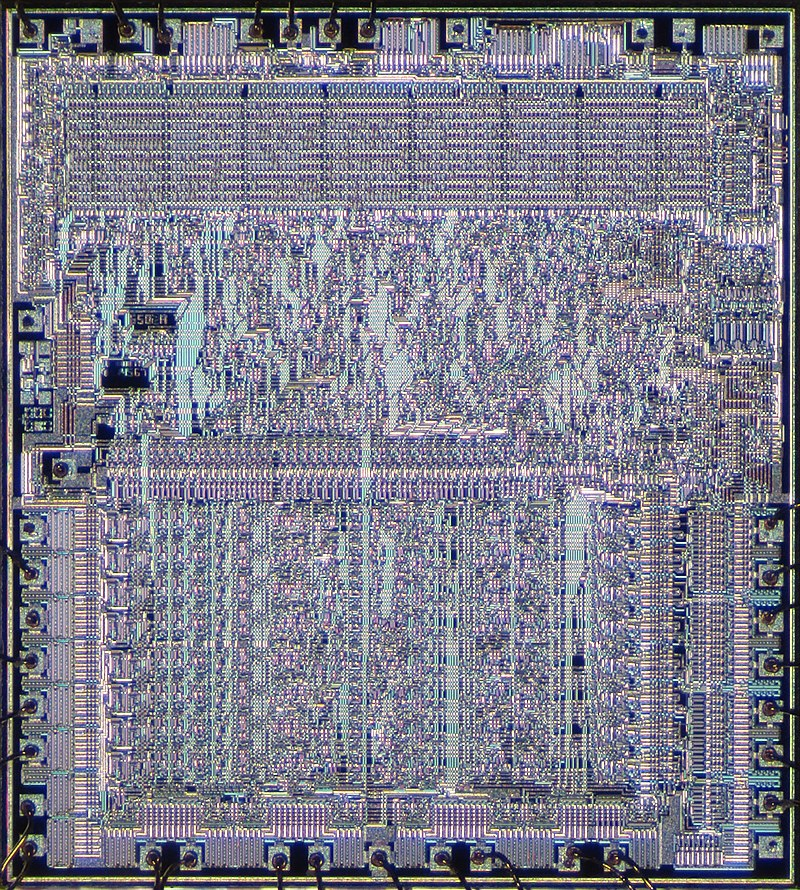
\includegraphics[width=0.85\textwidth,height=6cm,keepaspectratio]{image4.png}
            \par
            \vspace{0.5em}
    \end{columns}
\end{frame}

% --- SECTION 2 ---
\section{Computing at Scale}

\begin{frame}{Scaling Laws}
    \textbf{Moore's Law}:
    Transistor count per microprocessor doubles every $\approx$2 years.

    \vspace{1em}
    \textbf{Dennard Scaling}:
    \begin{itemize}
        \item Power density stays constant as transistors shrink.
        \item Same chip area $\to$ Same power draw.
    \end{itemize}

    \vspace{1em}
    \centering
    \alert{\textit{These trends drove decades of progress.}}
\end{frame}

\begin{frame}{50 Years of Trends}
    % Full slide graphic for impact
    \begin{figure}
        \centering
        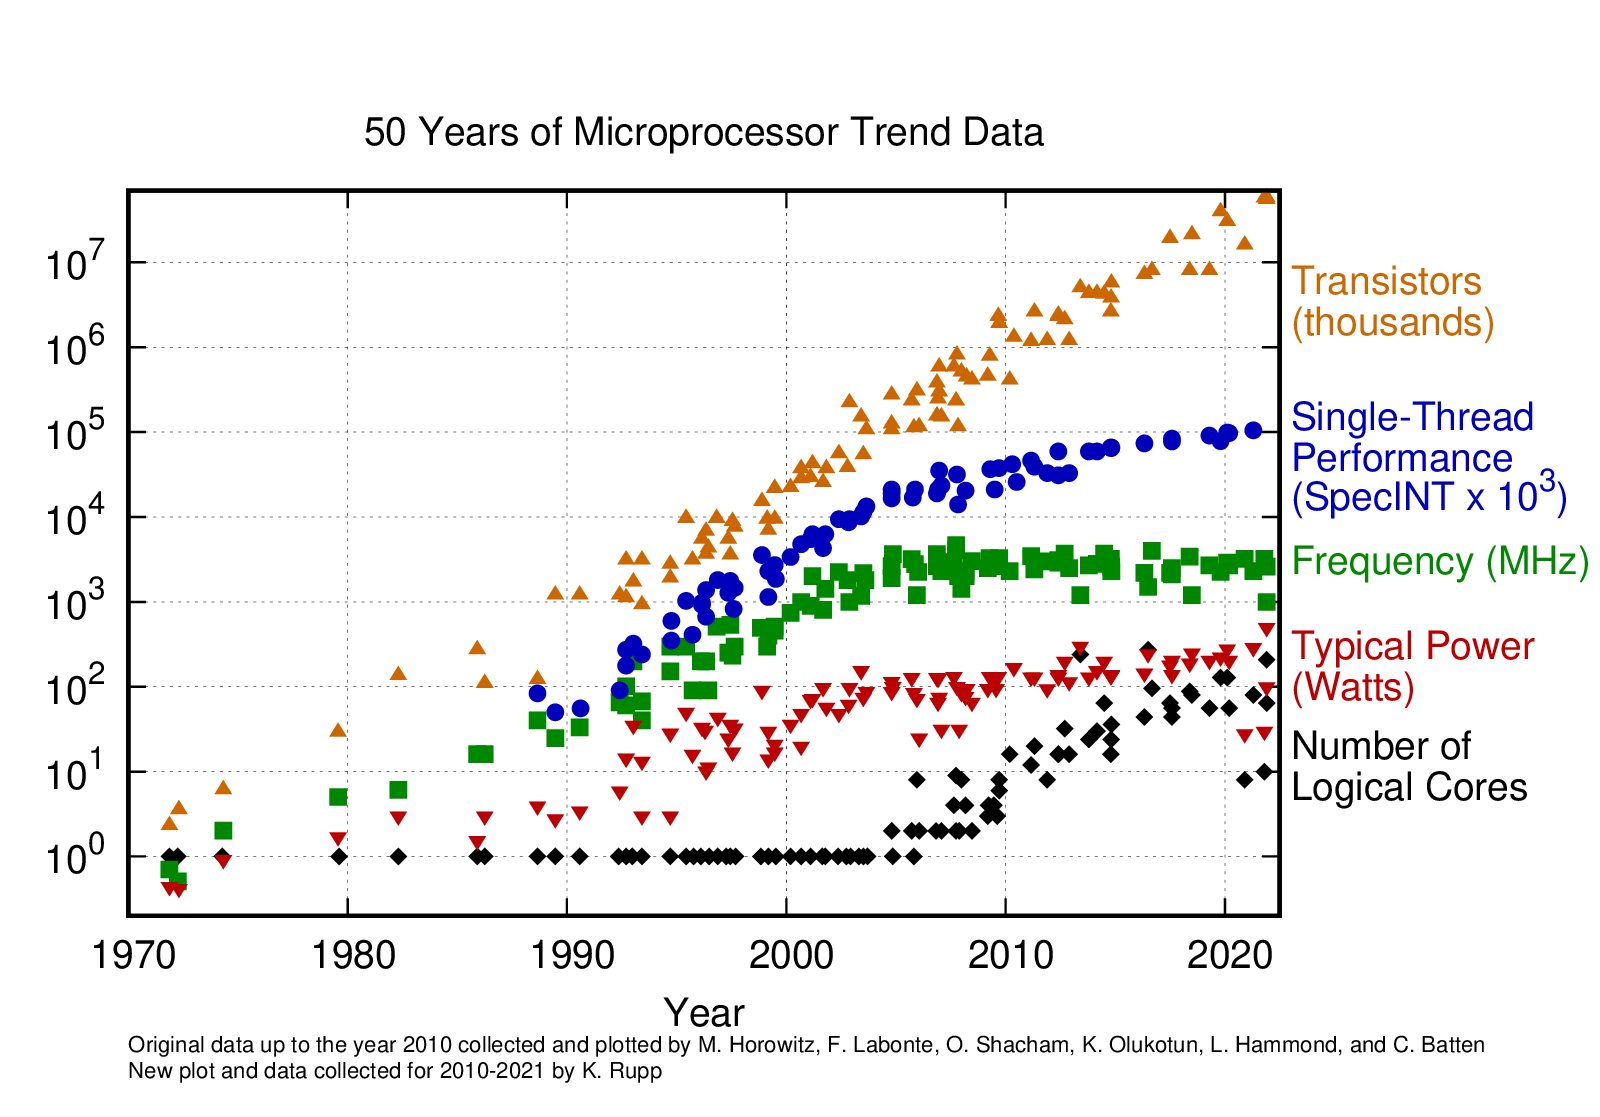
\includegraphics[width=0.9\textwidth,height=6.8cm,keepaspectratio]{image2.png}
        \caption{Transistors, Frequency, Power, and Cores (1970--2020)}
    \end{figure}
\end{frame}

\begin{frame}{Wafer-Scale Engines}
    Making bigger chips. From reticle-sized to wafer-sized.

    % \vspace{1em}
    % \begin{columns}[T, onlytextwidth]
    %     \column{0.45\textwidth}
    %         \textbf{Standard GPU}
    %         \begin{itemize}
    %             \item 54.2 Billion Transistors
    %             \item $826~mm^{2}$ Silicon
    %         \end{itemize}

    %     \column{0.45\textwidth}
    %         \textbf{Cerebras WSE-2}
    %         \begin{itemize}
    %             \item \alert{2.6 Trillion} Transistors
    %             \item \alert{$46,225~mm^{2}$} Silicon
    %         \end{itemize}
    % \end{columns}
    \vspace{1em}
    \centering
    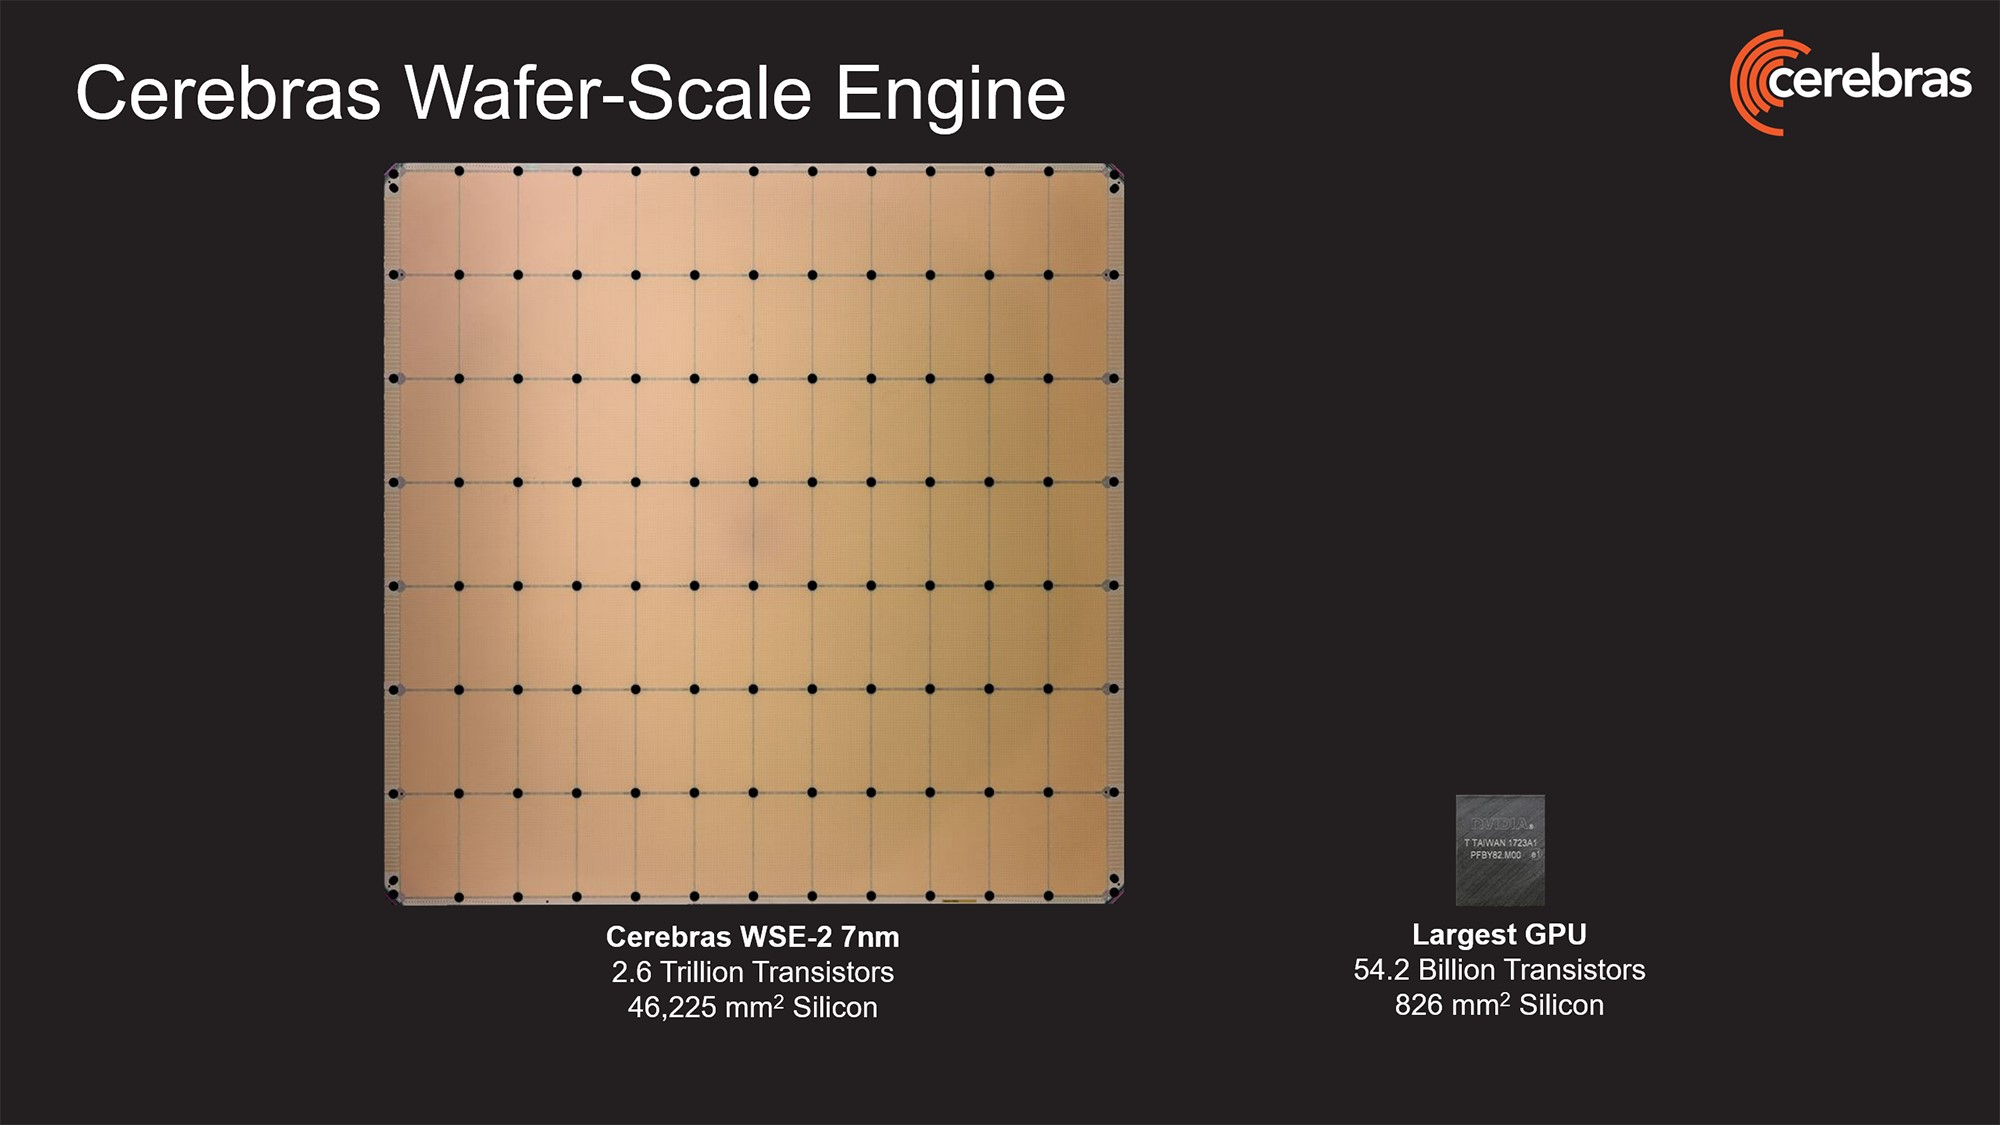
\includegraphics[width=0.9\textwidth,height=7cm,keepaspectratio]{image3.png}
\end{frame}

\begin{frame}{Beyond the Chip}
    Scale isn't just on-chip. It's the whole system.
    % \vspace{0.1em}

    Transistors $\to$ Chips $\to$ Boards $\to$ Racks $\to$ Aisles $\to$ Datacenters.

    \vspace{0.5em}
    \centering
    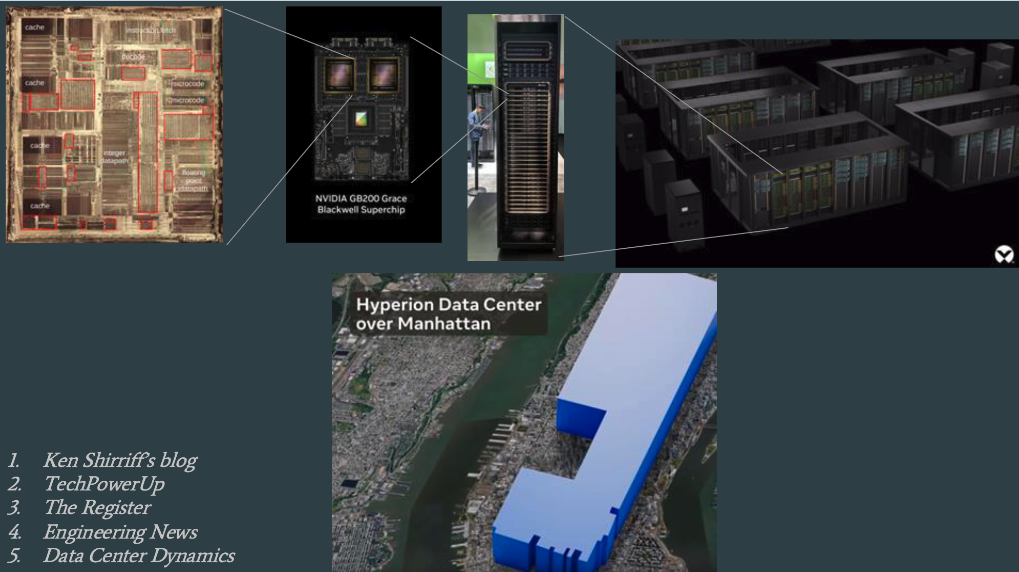
\includegraphics[width=0.95\textwidth,height=6cm,keepaspectratio]{hierarchy_of_computing_scale.png}
\end{frame}

\begin{frame}{The Scales of Computing}
    \centering
    We scaled transistors \textbf{down}, and hit hard physical limits.

    We scaled \textbf{up} and made bigger chips.

    We connected more chips together and scaled \textbf{out}.

    Now even a single datacenter is too small, and we scale \textbf{across}.
\end{frame}

% --- SECTION 3 ---
\section{Impact: Power \& Water}

\begin{frame}{Unprecedented Energy Scale}
    \begin{columns}[c, onlytextwidth]
        \column{0.6\textwidth}
            \textbf{The Jump in Scale}
            \begin{itemize}
                \item \textbf{Past:} Top supercomputers $\approx$ 20 MW
                \item \textbf{Future:} Meta's ``Hyperion'' DC $\approx$ \alert{5 GW}.
                \item Note: A nuclear plant outputs $\approx 1$ GW.
            \end{itemize}

        \column{0.5\textwidth}
            \centering
            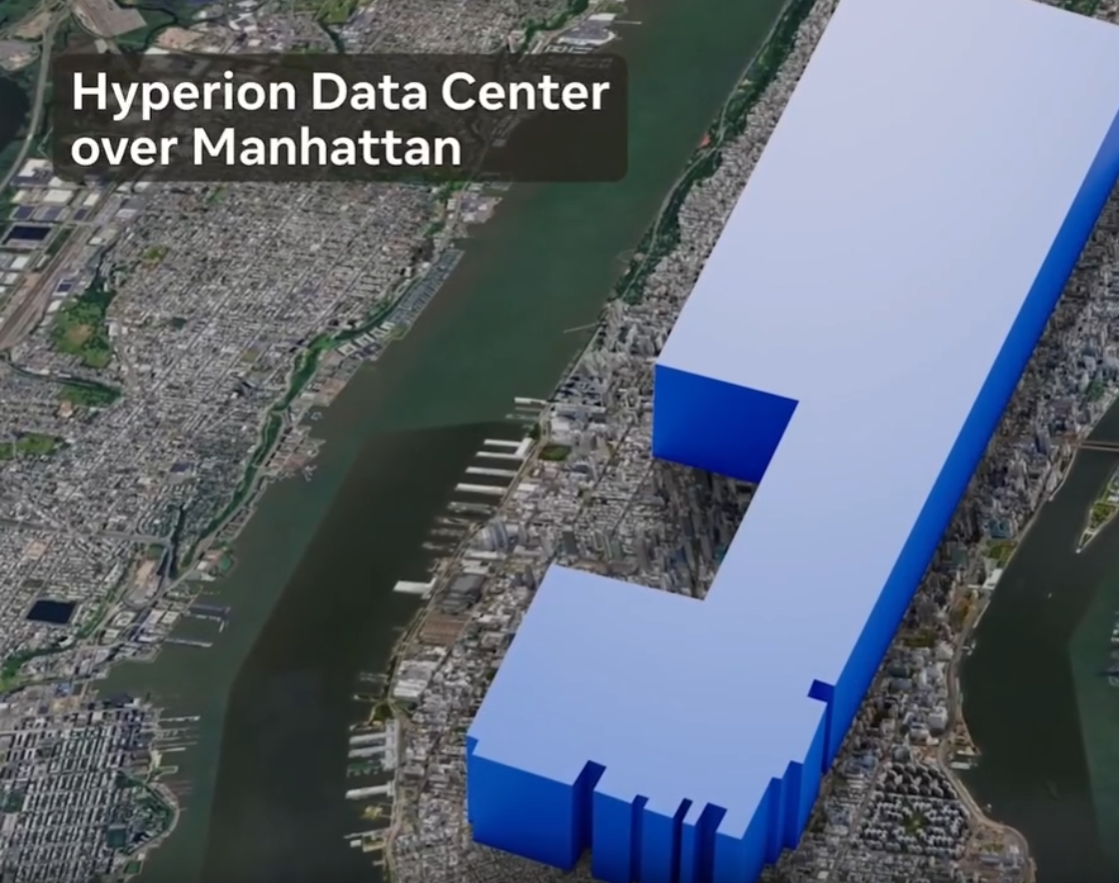
\includegraphics[width=\textwidth,height=4.8cm,keepaspectratio]{image10.png}
            \par
            \scriptsize{Hyperion Data Center scale over Manhattan}
    \end{columns}
\end{frame}

\begin{frame}{The Strain on our Energy Grid.}
    \begin{columns}[c, onlytextwidth]
        \column{0.45\textwidth}
            \begin{itemize}
                \item Demand is outstripping generation capacity.
                \item Demand spiked \alert{rapidly}. Decadal planning $\rightarrow$ ASAP.
                \item AI training loads can fluctuate 100s of MWs in seconds.
                \item Inflated demand through speculation and multiple bids
                \item AI bubble?
                % \item \textit{See Right:} Georgia Power's projected winter peak demand.
            \end{itemize}

        \column{0.55\textwidth}
            \centering
            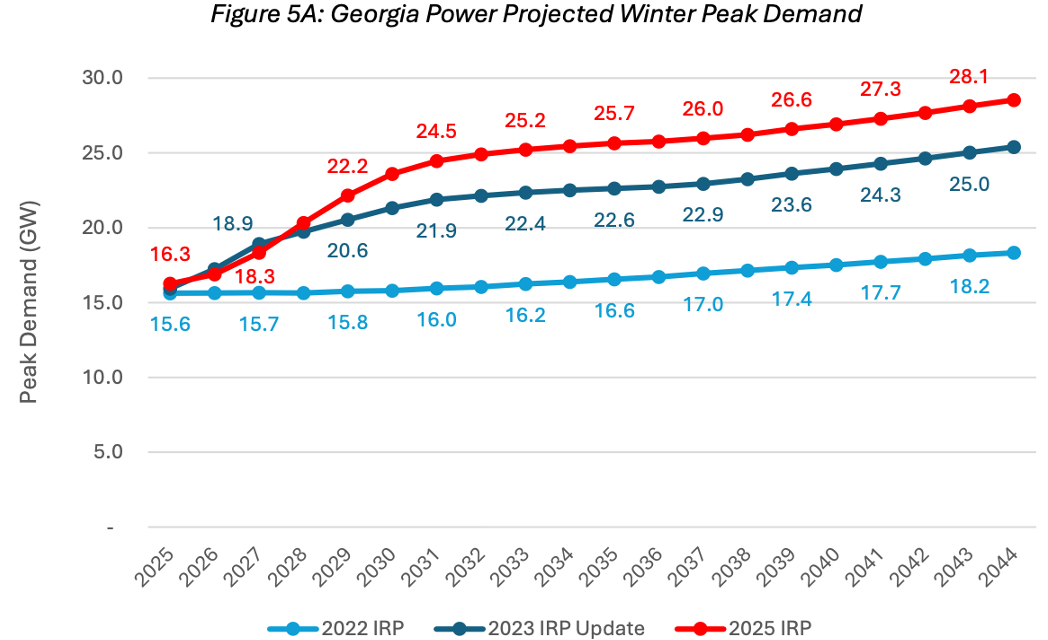
\includegraphics[width=\textwidth,height=5.5cm,keepaspectratio]{image12.png}
            \par
            \scriptsize{Source: Georgia Power IRP}
    \end{columns}
\end{frame}

\begin{frame}{The Water Cost}
    \textbf{Massive Power + Inefficiencies = Cooling Demand}

    \begin{block}{The Cost of Evaporative Cooling}
        \begin{itemize}
            \item Evaporative cooling is very effective and power-efficient, but not without tradeoffs.
            \item A single DC \textit{can} evaporate millions of gallons of water/day.
            \item Equivalent to the usage of hundreds of thousands of people.
            \item Can be mitigated by: free-air/dry/adiabatic cooling, water reuse, etc.
        \end{itemize}
    \end{block}

    \vspace{1em}
    \textbf{Secondary Water Impact:} Thermoelectric power generation (for the electricity the DC uses) is already the largest water consumer in the US.
\end{frame}


% --- SECTION 4 ---
\section{The Future}

\begin{frame}{In Space and Under the Sea}
    We're reconsidering the environments computing operates in.

    Both extremes are being actively tested.

    \vspace{1em}
    % Two columns, one for space and one for sea
    \begin{columns}[c, onlytextwidth]
        \column{0.5\textwidth}
            \textbf{Space}
            \begin{itemize}
                \item Solar energy availability
                \item Cooling challenges
                \item Radiation/error tolerance
                \item Cost of deployment and repairs
                \item Inter-satellite communication
            \end{itemize}
        \column{0.5\textwidth}
            \textbf{Sea}
            \begin{itemize}
                \item Water availability
                \item Environmental effects
                \item Cost of deployment and repairs
            \end{itemize}
    \end{columns}

\end{frame}


\begin{frame}{Limits of Scale/Computing}
    \begin{columns}[c, onlytextwidth]
        \column{0.55\textwidth}
            What is the limit of computing at scale?\\[1.5em]
            Is there a limit?\\[1.5em]
            Should we self-impose a limit?
        \column{0.45\textwidth}
            \centering
            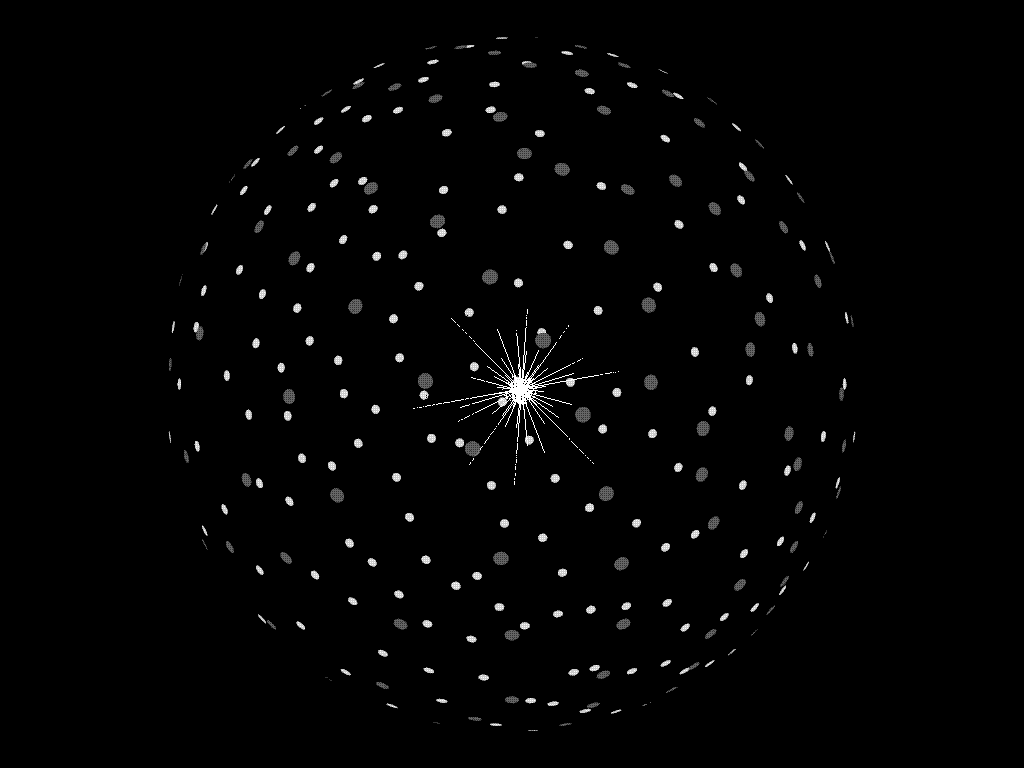
\includegraphics[width=\textwidth,keepaspectratio]{images/matrioshka_brain_wiki.png}
            \par
            \scriptsize{Artistic depiction of a Matrioshka Brain}
    \end{columns}
\end{frame}


% \begin{frame}{Efficiency and Jevons Paradox}

%     \textbf{Efficiency:} What if we just made everything more efficient?

%     \textbf{Jevons Paradox:} Increasing resource efficiency induces increased demand and overall resource consumption.

%     \begin{itemize}
%         \item We have 70 years of data showing this in computing.
%         \item Alternative: Lighting (candles $\to$ LEDs) is capped by biology.
%     \end{itemize}

% \end{frame}

\begin{frame}{Efficiency and Jevons Paradox}

    \begin{itemize}
        \item \textbf{The Efficiency Trend (Koomey's Law):}
        \begin{itemize}
            \item Computations per joule doubled every $\approx 1.57$ years for decades (now slower).
            \item \textit{Result:} Modern computers are vastly more efficient than their predecessors.
        \end{itemize}

        \vspace{0.3cm} % Adds a little breathing room

        \item \textbf{Jevons Paradox:}
        \begin{itemize}
            \item Efficiency improvements induce increased demand and overall resource consumption.
            \item Gains in computing efficiency unlock new applications and demand (e.g. we now use AI for internet searches).
        \end{itemize}
    \end{itemize}

    % \vspace{0.5cm}

    % Using a block makes the key takeaway stand out
    \begin{block}{The Divergence}
        \begin{itemize}
            \item \textbf{Lighting Demand:} Capped by biology/physics (e.g., the human eye).
            \item \textbf{Computing Demand:} Capped only by available energy and heat dissipation?
        \end{itemize}
        \centering
    \end{block}
    \textbf{Will gains in computing efficiency lead to reduced resource consumption?}


\end{frame}

\begin{frame}{Sufficiency, Sobriety, and Ethics}
    \textbf{Sufficiency:} What is the least amount of resources/computing to complete a task?
    \begin{itemize}
        \item Example: Can I use a linear regression or do I need a 1 trillion parameter model?
        \item \textbf{Self}-sufficiency example: Solar-powered pocket calculator
    \end{itemize}
    \textbf{Sobriety:} Is this a problem I need (computing) to solve?
    \begin{itemize}
        \item Conscious evaluation of tech use. \textbf{Re-examine our relationship with technology.}
        \item Example: Does my toaster need AI to make my morning toast?
    \end{itemize}
    \textbf{Ethics:} How do we ensure computing systems at scale are ethically designed, built, operated, used, and decommissioned?
\end{frame}


\begin{frame}{Summary: Computing at Scale}
    The full stack of computing at scale:

    \vspace{0.5em}

    \begin{enumerate}
        \item \textbf{The Foundation:} Information processing is valuable, and we use physical computers to perform this task.
        \item \textbf{The Engine:} Transistors drove 50 years of exponential growth (Moore/Dennard), but are hitting lower limits.
        \item \textbf{The New Scale:} We now scale up, out, and across to form massive systems (datacenters).
        \item \textbf{The Constraint:} This massive scale is colliding with physical realities: energy grids, water supplies, and communities (us).
    \end{enumerate}

    % \vspace{0.5em}

    % \begin{alertblock}{The Core Question}
    % \end{alertblock}
\end{frame}


% --- STANDOUT FRAME FOR CONCLUSION ---
\begin{frame}[standout]
    \centering

    % The Premise: Medium size, with color emphasis on the opposing concepts
    \large
    Our technical ability to scale is \alert{limitless},\\
    but our resources and ethical boundaries are \alert{limited}.

    \vspace{3em} % Significant whitespace for dramatic pause

    % The Challenge: Huge size, italicized "you" for direct engagement
    \Huge
    What do \textit{you} want the future\\[0.2em]
    of computing to look like?

\end{frame}

\end{document}
